\chapter{Hamiltonian Mechanics}\label{ch:b3:hamiltonian-mechanics}

Photograph a pendulum a thousand times and plot, for each shot, its
angle against its angular momentum: the points fall on a closed curve,
and every possible motion of the pendulum is one such curve --- small
swings on nested ovals, full turns on wavy lines above and below, and
between them a single crossed curve separating the two regimes. This
picture, the \emph{\omterm{def:b3:hamiltonian-mechanics:portrait}{phase portrait}}, is the heart of the reformulation
Hamilton gave to mechanics in 1833: the state of a system is a point
in the space of coordinates \emph{and} momenta, its evolution is a
flow in that space, and the flow is generated by a single function,
the energy, through two beautifully symmetric first-order equations.
The reward is not easier calculations --- Lagrange usually wins there
--- but the right \emph{geometry}: the flow conserves phase-space
volume, which will found statistical physics; and its algebraic
skeleton, the \omterm{def:b3:hamiltonian-mechanics:poisson}{Poisson bracket}, is precisely what quantum mechanics
will promote into the commutator. This chapter is the hinge between
the mechanics of things and the physics of the twentieth century.

\section{From Lagrange to Hamilton}

\begin{definition}[Hamiltonian and canonical equations]\label{def:b3:hamiltonian-mechanics:hamiltonian}
\index{Hamiltonian}\index{canonical equations}\index{phase space}
For a system with \omterm{def:b3:lagrangian-mechanics:action}{Lagrangian} $L(q, \dot q, t)$, express the velocities
in terms of the momenta $p_i = \partial L/\partial\dot q_i$ and define
the \emph{Hamiltonian} as the Legendre transform
\[
H(q, p, t) = \sum_i p_i\dot q_i - L ,
\]
a function of the coordinates and the \emph{momenta}. The
$2n$-dimensional space of the $(q_1, \dots, q_n, p_1, \dots, p_n)$ is
the \emph{phase space}; one point of it --- one \emph{state} ---
determines the entire future and past of the system through the
\emph{canonical equations} of
\cref{thm:b3:hamiltonian-mechanics:canonical}.
\end{definition}

\begin{theorem}[Hamilton's equations]\label{thm:b3:hamiltonian-mechanics:canonical}
The \omterm{thm:b3:lagrangian-mechanics:euler-lagrange}{Euler--Lagrange equations} are equivalent to the $2n$ first-order
equations
\[
\dot q_i = \frac{\partial H}{\partial p_i} , \qquad
\dot p_i = -\frac{\partial H}{\partial q_i} .
\]
\end{theorem}

\begin{proof}
Differentiate $H = \sum p_i\dot q_i - L$ as a function of $(q, p, t)$:
$\dd H = \sum(\dot q_i\,\dd p_i + p_i\,\dd\dot q_i) - \sum(
\partial_{q_i}L\,\dd q_i + \partial_{\dot q_i}L\,\dd\dot q_i) -
\partial_tL\,\dd t$. The $\dd\dot q_i$ terms cancel by the definition
of $p_i$ --- the whole point of the Legendre transform --- leaving
$\dd H = \sum(\dot q_i\,\dd p_i - \partial_{q_i}L\,\dd q_i) -
\partial_tL\,\dd t$. Reading off the partial derivatives:
$\partial H/\partial p_i = \dot q_i$ and $\partial H/\partial q_i =
-\partial L/\partial q_i$, which by Euler--Lagrange is $-\dot p_i$.
(Also $\partial_tH = -\partial_tL$.)
\end{proof}

\begin{proposition}[What $H$ is]\label{prop:b3:hamiltonian-mechanics:energy}
$H$ coincides with the \omterm{prop:b3:lagrangian-mechanics:energy}{energy function} $h$ of the previous chapter:
along a motion, $\dd H/\dd t = \partial H/\partial t$, so $H$ is
conserved whenever it has no explicit time dependence; and when the
kinetic energy is quadratic in the velocities with time-independent
\omterm{def:b3:lagrangian-mechanics:coordinates}{constraints}, $H = E_k + E_p$, the mechanical energy --- now written in
the variables $(q, p)$.
\end{proposition}

\begin{proof}
$\dd H/\dd t = \sum(\partial_{q_i}H\,\dot q_i + \partial_{p_i}H\,\dot
p_i) + \partial_tH = \sum(\partial_{q_i}H\,\partial_{p_i}H -
\partial_{p_i}H\,\partial_{q_i}H) + \partial_tH = \partial_tH$: the
symmetry of the \omterm{def:b3:hamiltonian-mechanics:hamiltonian}{canonical equations} makes the sum cancel identically.
The identification with $E_k + E_p$ is
\cref{prop:b3:lagrangian-mechanics:energy}.
\end{proof}

\begin{example}[Two Hamiltonians]\label{ex:b3:hamiltonian-mechanics:examples}
Mass on a spring: $p = m\dot x$, so
\[
H = \frac{p^2}{2m} + \frac12 kx^2 ;
\]
the \omterm{def:b3:hamiltonian-mechanics:hamiltonian}{canonical equations} $\dot x = p/m$, $\dot p = -kx$ are the familiar
pair. Pendulum: $p = m\ell^2\dot\theta$ and
\[
H = \frac{p^2}{2m\ell^2} - mg\ell\cos\theta .
\]
In both cases $H$ is the energy, constant on each motion: the motions
\emph{are} the level curves of $H$ in the $(q,p)$ plane.
\end{example}

\begin{method}[The Hamiltonian recipe]\label{met:b3:hamiltonian-mechanics:recipe}
(1) From $L$, compute the momenta $p_i = \partial L/\partial\dot q_i$
and invert for the $\dot q_i$. (2) $H = \sum p_i\dot q_i - L$,
expressed in $(q, p)$ only --- for a natural system, simply $E_k + E_p$
with $E_k$ rewritten in the momenta. (3) Write the \omterm{def:b3:hamiltonian-mechanics:hamiltonian}{canonical
equations}. (4) Draw the level curves of $H$: for one degree of
freedom they are the trajectories, and the whole qualitative motion
--- oscillations, rotations, equilibria, separatrices --- is read off
without solving anything.
\end{method}

\section{Phase space}

\begin{definition}[Phase portrait, fixed points, separatrix]\label{def:b3:hamiltonian-mechanics:portrait}
\index{phase portrait}\index{fixed point}\index{separatrix}
The \emph{phase portrait} of a system is the family of its
trajectories in \omterm{def:b3:hamiltonian-mechanics:hamiltonian}{phase space}. A \emph{fixed point} is a state where
both \omterm{def:b3:hamiltonian-mechanics:hamiltonian}{canonical equations} vanish --- an equilibrium: a minimum of the
potential appears as a \emph{centre} surrounded by closed curves, a
maximum as a \emph{saddle} through which passes a \emph{separatrix},
the trajectory that divides \omterm{def:b3:hamiltonian-mechanics:hamiltonian}{phase space} into regions of qualitatively
different motion.
\end{definition}

\begin{example}[The pendulum's phase portrait]\label{ex:b3:hamiltonian-mechanics:pendulum-portrait}
For $H = p^2/2m\ell^2 - mg\ell\cos\theta$: closed ovals around
$(0, 0)$ --- \emph{librations}, the ordinary swings; wavy curves at
$|p|$ large --- \emph{rotations}, the pendulum turning over the top;
and through the saddles at $\theta = \pm\pi$ the \omterm{def:b3:hamiltonian-mechanics:portrait}{separatrix}, of energy
$E = +mg\ell$, on which the pendulum takes an infinite time to reach
the top. A state on the \omterm{def:b3:hamiltonian-mechanics:portrait}{separatrix} is the swing launched \emph{exactly}
hard enough to arrive at the inverted position with nothing to spare.
\end{example}

\begin{omfigure}
\begin{tikzpicture}
  \begin{axis}[omaxis, axis x line=bottom, axis y line=left,
    width=11.6cm, height=6.4cm, xmin=-180, xmax=180, ymin=-3.2, ymax=3.2,
    xlabel={$\theta$ (degrees)},
    xlabel style={at={(axis description cs:0.5,-0.08)}, anchor=north},
    ylabel={$p$ (units of $m\ell^2\omega_0$)},
    xtick={-180,-90,0,90,180}, ytick={-2,0,2}, clip=false]
    % librations E/mgl = -0.5 and 0.4 : p = ±sqrt(2(E'+cos x)), E'=E/mgl
    \addplot[omDef, thick, domain=-60:60, samples=80] {sqrt(2*(-0.5+cos(x)))};
    \addplot[omDef, thick, domain=-60:60, samples=80] {-sqrt(2*(-0.5+cos(x)))};
    \addplot[omDef, thick, domain=-113.5:113.5, samples=100] {sqrt(2*(0.4+cos(x)))};
    \addplot[omDef, thick, domain=-113.5:113.5, samples=100] {-sqrt(2*(0.4+cos(x)))};
    % separatrix E'=1: p=±2cos(x/2)
    \addplot[omThm, very thick, domain=-180:180, samples=100] {2*cos(x/2)};
    \addplot[omThm, very thick, domain=-180:180, samples=100] {-2*cos(x/2)};
    % rotations E'=2 and 3.5
    \addplot[omExo, thick, domain=-180:180, samples=100] {sqrt(2*(2+cos(x)))};
    \addplot[omExo, thick, domain=-180:180, samples=100] {-sqrt(2*(2+cos(x)))};
    \addplot[omExo, thick, domain=-180:180, samples=100] {sqrt(2*(3.5+cos(x)))};
    \addplot[omExo, thick, domain=-180:180, samples=100] {-sqrt(2*(3.5+cos(x)))};
    % fixed points
    \fill (axis cs:0,0) circle (1.8pt);
    \fill (axis cs:180,0) circle (1.8pt);
    \fill (axis cs:-180,0) circle (1.8pt);
    % flow arrows
    \draw[->, thick] (axis cs:-6,1.66) -- (axis cs:6,1.66);
    \draw[->, thick] (axis cs:6,-1.66) -- (axis cs:-6,-1.66);
    \draw[->, thick] (axis cs:-6,2.45) -- (axis cs:6,2.45);
    \draw[->, thick] (axis cs:6,-2.45) -- (axis cs:-6,-2.45);
    \node[omDef, font=\scriptsize, anchor=west] at (axis cs:-52,0.5) {libration};
    \node[omThm, font=\scriptsize, anchor=west] at (axis cs:97,1.75) {separatrix};
    \node[omExo, font=\scriptsize, anchor=west] at (axis cs:-172,2.93) {rotation};
  \end{axis}
\end{tikzpicture}

{\small The pendulum's \omterm{def:b3:hamiltonian-mechanics:portrait}{phase portrait}: level curves of $H$. Closed
ovals (swings) circulate clockwise around the centre; above and below
the \omterm{def:b3:hamiltonian-mechanics:portrait}{separatrix}, the pendulum rotates. The saddles at $\pm 180^\circ$
are the inverted equilibrium.}
\end{omfigure}

\begin{theorem}[Liouville's theorem]\label{thm:b3:hamiltonian-mechanics:liouville}
\index{Liouville's theorem}
The \omterm{def:b3:hamiltonian-mechanics:hamiltonian}{Hamiltonian} flow preserves phase-space volume: if a region of
initial states is carried along by the \omterm{def:b3:hamiltonian-mechanics:hamiltonian}{canonical equations}, its volume
(its area, for one degree of freedom) never changes --- whatever its
shape becomes.
\end{theorem}

\begin{proof}
The flow in \omterm{def:b3:hamiltonian-mechanics:hamiltonian}{phase space} has velocity field $(\dot q_i, \dot p_i) =
(\partial_{p_i}H, -\partial_{q_i}H)$. Its divergence is
\[
\sum_i\Big(\frac{\partial\dot q_i}{\partial q_i}
 + \frac{\partial\dot p_i}{\partial p_i}\Big)
 = \sum_i\Big(\frac{\partial^2H}{\partial q_i\partial p_i}
 - \frac{\partial^2H}{\partial p_i\partial q_i}\Big) = 0 :
\]
the flow is incompressible, and an incompressible flow transports
volumes unchanged, as for the fluids of the Year 2 volume. (The
formal step from zero divergence to conserved volume is the transport
theorem proved there.)
\end{proof}

\begin{remark}[Why Liouville matters]\label{rem:b3:hamiltonian-mechanics:liouville-matters}
Nothing in Newton's formulation suggests that anything is
incompressible. In the \omterm{def:b3:hamiltonian-mechanics:hamiltonian}{Hamiltonian} picture it is automatic --- and it
is the licence for statistical physics: when we describe a gas of
$10^{23}$ molecules by a cloud of points in \omterm{def:b3:hamiltonian-mechanics:hamiltonian}{phase space}, Liouville's
theorem says the cloud flows like an incompressible fluid, so
``number of states in a phase-space volume'' is a quantity dynamics
itself cannot create or destroy. The microcanonical postulate of
statistical physics, later in this volume, stands on exactly this.
\end{remark}

\begin{omfigure}
\begin{tikzpicture}[font=\small, >=Stealth]
  % free particle shear
  \begin{scope}
    \draw[->] (0,0) -- (5.2,0) node[right] {$q$};
    \draw[->] (0,0) -- (0,3.0) node[above] {$p$};
    \fill[omDef!30, draw=omDef, thick] (0.6,0.8) rectangle (1.6,2.2);
    \fill[omDef!30, draw=omDef, thick] (2.7,0.8) -- (3.7,0.8) -- (5.1,2.2) -- (4.1,2.2) -- cycle;
    \draw[->, thick] (1.85,1.5) -- (2.5,1.5);
    \node at (1.1,0.45) {$t = 0$};
    \node at (3.9,0.45) {$t > 0$};
  \end{scope}
  \node[font=\footnotesize] at (2.6,-0.7) {free particle: $\dot q = p/m$ shears the blob};
  % harmonic oscillator rotation
  \begin{scope}[xshift=9.6cm]
    \draw[->] (-2.6,0) -- (2.8,0) node[right] {$q$};
    \draw[->] (0,-1.55) -- (0,2.9) node[above] {$p$};
    \draw[gray, dashed] (0,0) circle (1.75);
    \fill[omThm!30, draw=omThm, thick] (1.35,0.35) -- (2.15,0.35) -- (2.15,0.95) -- (1.35,0.95) -- cycle;
    \begin{scope}[rotate=100]
    \fill[omThm!30, draw=omThm, thick] (1.35,0.35) -- (2.15,0.35) -- (2.15,0.95) -- (1.35,0.95) -- cycle;
    \end{scope}
    \draw[->, thick] (2.0,1.35) arc (35:75:2.35);
    \node at (2.5,-0.45) {$t = 0$};
    \node at (-1.15,2.45) {$t > 0$};
  \end{scope}
  \node[font=\footnotesize] at (9.6,-0.7) {harmonic oscillator: the blob turns rigidly};
\end{tikzpicture}

{\small Liouville's theorem: the flow deforms a region of initial
states --- shearing it, turning it --- but its area is exactly
conserved.}
\end{omfigure}

\section{Poisson brackets}

\begin{definition}[Poisson bracket]\label{def:b3:hamiltonian-mechanics:poisson}
\index{Poisson bracket}
The \emph{Poisson bracket} of two functions $f(q, p, t)$ and
$g(q, p, t)$ on \omterm{def:b3:hamiltonian-mechanics:hamiltonian}{phase space} is
\[
\{f, g\} = \sum_i\Big(
 \frac{\partial f}{\partial q_i}\frac{\partial g}{\partial p_i}
 - \frac{\partial f}{\partial p_i}\frac{\partial g}{\partial q_i}\Big) .
\]
It is antisymmetric, linear in each argument, obeys the product rule
$\{f, gh\} = \{f, g\}h + g\{f, h\}$, and satisfies for the coordinates
themselves the \emph{canonical relations}
\[
\{q_i, p_j\} = \delta_{ij} , \qquad
\{q_i, q_j\} = \{p_i, p_j\} = 0 .
\]
\end{definition}

\begin{theorem}[Evolution as a bracket]\label{thm:b3:hamiltonian-mechanics:evolution}
Along any motion,
\[
\frac{\dd f}{\dd t} = \{f, H\} + \frac{\partial f}{\partial t} .
\]
In particular a quantity without explicit time dependence is conserved
if and only if its bracket with the \omterm{def:b3:hamiltonian-mechanics:hamiltonian}{Hamiltonian} vanishes; and the
\omterm{def:b3:hamiltonian-mechanics:hamiltonian}{canonical equations} themselves are $\dot q_i = \{q_i, H\}$, $\dot p_i
= \{p_i, H\}$: the \omterm{def:b3:hamiltonian-mechanics:hamiltonian}{Hamiltonian} \emph{generates} time evolution.
\end{theorem}

\begin{proof}
Chain rule plus the \omterm{def:b3:hamiltonian-mechanics:hamiltonian}{canonical equations}: $\dd f/\dd t = \sum(
\partial_{q_i}f\,\dot q_i + \partial_{p_i}f\,\dot p_i) + \partial_tf =
\sum(\partial_{q_i}f\,\partial_{p_i}H - \partial_{p_i}f\,
\partial_{q_i}H) + \partial_tf$.
\end{proof}

\begin{example}[Brackets of angular momentum]\label{ex:b3:hamiltonian-mechanics:brackets}
For one particle, $L_z = xp_y - yp_x$ and its cyclic companions. A
direct computation from the canonical relations gives
\[
\{L_x, L_y\} = L_z , \qquad
\{L_y, L_z\} = L_x , \qquad
\{L_z, L_x\} = L_y ,
\]
and $\{L^2, L_z\} = 0$: the components of angular momentum do not
``commute'' with each other, but each commutes with the total square.
Remember the shape of these relations --- they will return, verbatim,
as commutators in quantum mechanics, where they dictate everything
about atomic structure.
\end{example}

\begin{remark}[The doorway to quantum mechanics]\label{rem:b3:hamiltonian-mechanics:doorway}
Dirac observed in 1925 that the whole of quantum mechanics is obtained
by keeping the algebra of \omterm{def:b3:hamiltonian-mechanics:hamiltonian}{Hamiltonian} mechanics and replacing the
\omterm{def:b3:hamiltonian-mechanics:poisson}{Poisson bracket} by the commutator of operators divided by
$\iu\hbar$: $\{q, p\} = 1$ becomes $[\hat x, \hat p] = \iu\hbar$,
conservation is still ``bracket with $H$ vanishes'', and time
evolution is still generated by the \omterm{def:b3:hamiltonian-mechanics:hamiltonian}{Hamiltonian}. The classical theory
carries, in its bones, the skeleton of the quantum one; the chapters
on quantum mechanics will make this correspondence explicit.
\end{remark}

\section{Action and adiabatic invariants}

\begin{definition}[Action variable]\label{def:b3:hamiltonian-mechanics:action-variable}
\index{action variable}
For a one-degree-of-freedom system oscillating on a closed phase
trajectory, the \emph{\omterm{def:b3:lagrangian-mechanics:action}{action} variable} is the enclosed area divided by
$2\pi$:
\[
I = \frac{1}{2\pi}\oint p\,\dd q .
\]
\end{definition}

\begin{proposition}[Action of the harmonic oscillator]\label{prop:b3:hamiltonian-mechanics:sho-action}
For $H = p^2/2m + \tfrac12 m\omega^2q^2$ at energy $E$, the trajectory
is an ellipse of semi-axes $\sqrt{2E/m\omega^2}$ and $\sqrt{2mE}$,
enclosing the area $2\pi E/\omega$: hence
\[
I = \frac{E}{\omega} , \qquad E = \omega I ,
\]
and the oscillation frequency is $\partial E/\partial I = \omega$, as
it should be.
\end{proposition}

\begin{proof}
Area of an ellipse, $\pi ab = \pi\sqrt{2E/m\omega^2}\sqrt{2mE} =
2\pi E/\omega$.
\end{proof}

\begin{proposition}[Adiabatic invariance]\label{prop:b3:hamiltonian-mechanics:adiabatic}
\index{adiabatic invariant}
If a parameter of the system (a length, a stiffness, a field) is
varied \emph{slowly} --- over many oscillation periods --- the energy
changes, the frequency changes, but the \omterm{def:b3:lagrangian-mechanics:action}{action} $I$ stays constant to
an excellent approximation: $I$ is an \emph{\omterm{prop:b3:hamiltonian-mechanics:adiabatic}{adiabatic invariant}}. For
the slowly modified oscillator, $E/\omega$ is thus conserved: stiffen
the spring slowly to double $\omega$ and the energy doubles with it.
\end{proposition}

\begin{proof}[Partial proof]
For the oscillator with slowly varying $\omega(t)$: over one period
the work done by the changing parameter can be computed by averaging;
the calculation (guided in \cref{exo:b3:hamiltonian-mechanics:11})
gives $\dot E/E = \dot\omega/\omega$, i.e.\ $\dd(E/\omega)/\dd t = 0$
at leading order. The general statement, for any slowly deformed
oscillating system, is admitted --- it is the reason planetary orbits
survive slow perturbations, and the starting point of the ``old
quantum theory'' below.
\end{proof}

\begin{omfigure}
\begin{tikzpicture}[font=\small, >=Stealth]
  \begin{scope}
    \draw[->] (-2.9,0) -- (2.9,0) node[right] {$q$};
    \draw[->] (0,-1.9) -- (0,2.3) node[above] {$p$};
    \draw[omDef, thick] (0,0) ellipse (2.3 and 0.85);
    \draw[omThm, thick] (0,0) ellipse (1.63 and 1.2);
    \node[omDef, anchor=west] at (1.5,-1.1) {$\omega$};
    \node[omThm, anchor=west] at (0.2,1.45) {$2\omega$};
  \end{scope}
  \node[align=center] at (0,-2.75) {slowly stiffened oscillator:\\the ellipse narrows, the area survives};
  \begin{scope}[xshift=8.2cm]
    \fill (0,2.1) circle (1.5pt);
    \draw[thick] (-1.1,2.1) -- (1.1,2.1);
    \foreach \i in {-0.95,-0.6,-0.25,0.1,0.45,0.8} \draw (\i,2.1) -- (\i+0.16,2.24);
    \draw[thick] (0,2.1) -- ++(-115:1.15) coordinate (bob1);
    \fill[omDef] (bob1) circle (2.6pt);
    \draw[dashed] (0,2.1) -- ++(-115:2.3) coordinate (bob2);
    \fill[omDef!45] (bob2) circle (2.6pt);
    \draw[->] (0.02,1.0) -- (0.02,1.6);
    \node[anchor=west] at (0.1,1.28) {pull};
    \node[align=center] at (0,-0.85) {shortening a swinging pendulum slowly:\\$E/\omega$ constant, amplitude grows};
  \end{scope}
\end{tikzpicture}

{\small Adiabatic invariance. Left: as $\omega$ is slowly doubled, the
phase ellipse changes shape at constant area, so $E = \omega I$
doubles. Right: hoisting the string of a swinging pendulum feeds
energy into the swing in just the proportion that keeps
$I = E/\omega$ fixed.}
\end{omfigure}

\begin{remark}[The old quantum theory]\label{rem:b3:hamiltonian-mechanics:old-quantum}
Why do atoms have discrete energies? The first quantitative answer
(Bohr 1913, Sommerfeld 1915) was written in the language of this
chapter: among all classical motions, nature keeps those whose \omterm{def:b3:lagrangian-mechanics:action}{action}
integral is a whole number of Planck's constants,
\[
\oint p\,\dd q = nh .
\]
Applied to the harmonic oscillator this gives $E_n = n\hbar\omega$
(missing only the half of the true $\big(n + \tfrac12\big)\hbar
\omega$); applied to a particle in a box it gives \emph{exactly} the
levels of the Year 2 volume; applied to the hydrogen atom
(\cref{pb:b3:hamiltonian-mechanics:1}) it gives the measured spectrum
to four figures. The rule was quantitatively right and conceptually
provisional --- and because \omterm{def:b3:lagrangian-mechanics:action}{action} is an \omterm{prop:b3:hamiltonian-mechanics:adiabatic}{adiabatic invariant}, the
quantum number $n$ does not change under slow perturbations, which is
why such a rule could work at all. The true theory begins five
chapters from here.
\end{remark}

\begin{omfigure}
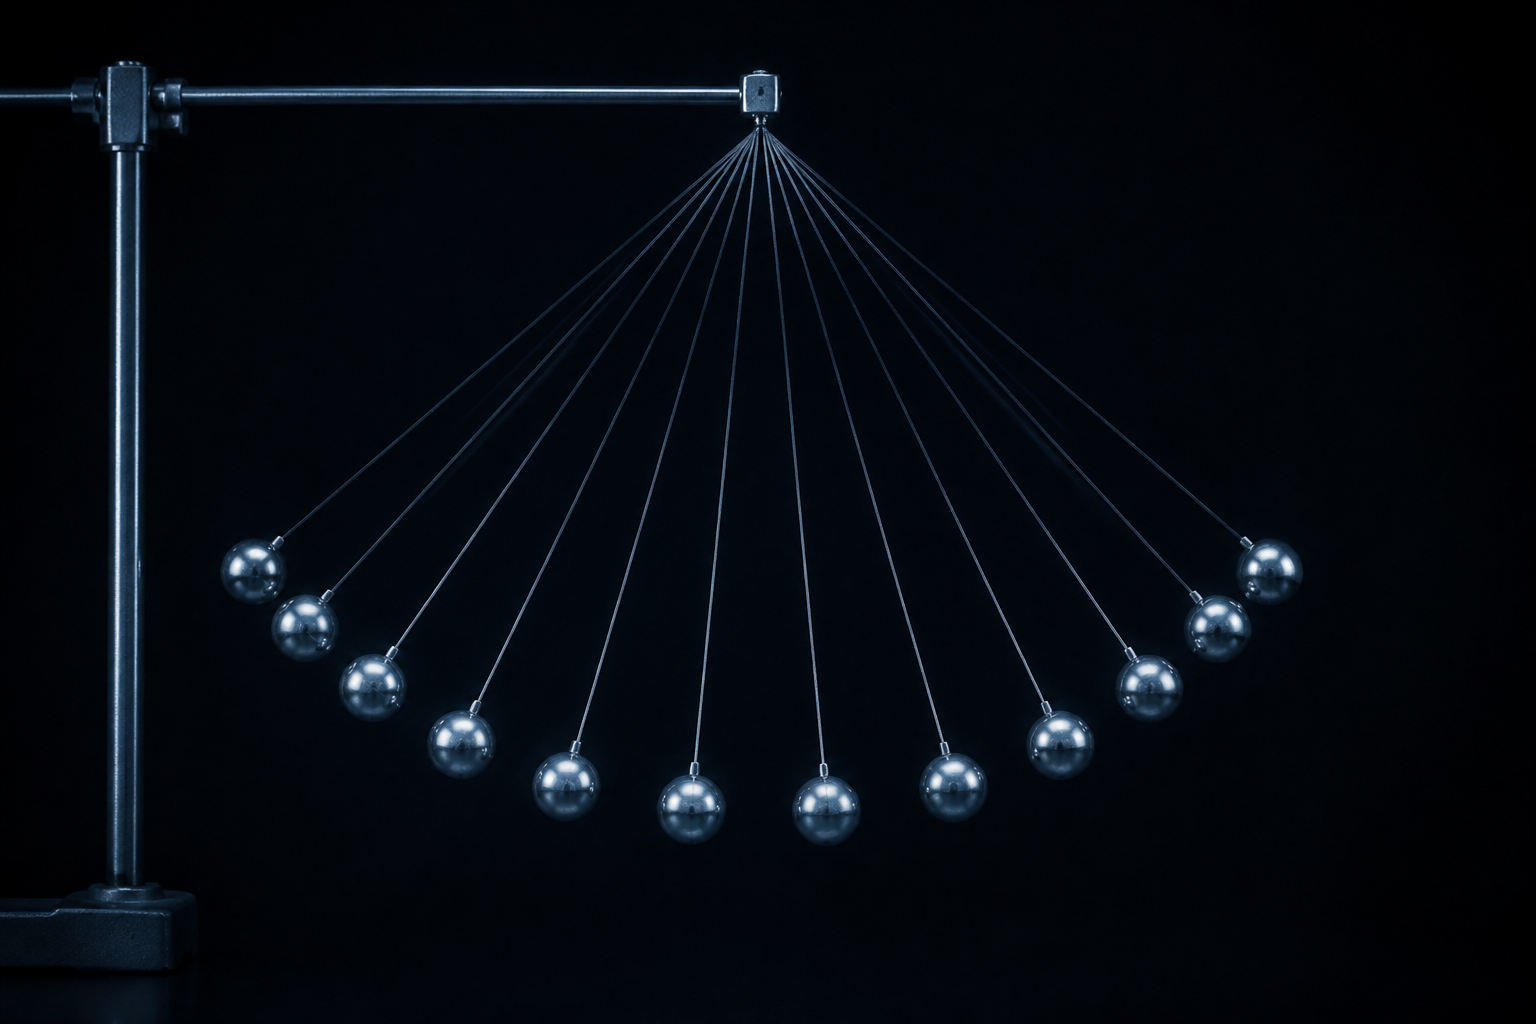
\includegraphics[width=0.58\linewidth]{images/book5/ai/b5-02-pendulum-strobe.png}

{\small A strobed pendulum: positions crowd near the turning points, where the bob lingers, and spread at the bottom, where it hurries --- a photograph of the phase-space portrait this chapter draws with equations.}
\end{omfigure}

\section{Exercises}

\begin{exercise}[$\star$]\label{exo:b3:hamiltonian-mechanics:1}
For the mass on a spring: (a) construct $H$ from $L$ and check $H =
E_k + E_p$; (b) write the \omterm{def:b3:hamiltonian-mechanics:hamiltonian}{canonical equations} and verify they
reproduce $\ddot x = -\omega^2x$; (c) show the trajectories are
ellipses in the $(x, p)$ plane and give their semi-axes at energy $E$;
(d) in what sense does the representative point move clockwise?
\end{exercise}

\begin{exercise}[$\star$]\label{exo:b3:hamiltonian-mechanics:2}
The bead on the rotating hoop of the previous chapter has $L =
\tfrac12 mR^2\dot\theta^2 + \tfrac12 m\omega^2R^2\sin^2\theta +
mgR\cos\theta$. (a) Compute $p$ and $H$. (b) Is $H$ conserved? Is it
the mechanical energy? (c) Sketch the level curves of $H$ for
$\omega^2 < g/R$ and $\omega^2 > g/R$, using the effective potential
of that chapter. (d) Identify the centres, the saddles and the
separatrices in the fast case.
\end{exercise}

\begin{exercise}[$\star$]\label{exo:b3:hamiltonian-mechanics:3}
A ball bounces elastically on the floor, $H = p^2/2m + mgz$ ($z >
0$). (a) Draw the phase trajectory for one flight and the whole
bouncing motion. (b) What does the elastic bounce do to the
representative point? (c) Compute the enclosed area for maximum height
$z_{\max}$, and the \omterm{def:b3:lagrangian-mechanics:action}{action} $I$. (d) The Bohr--Sommerfeld rule
$\oint p\,\dd z = nh$ applied to a bouncing neutron ($m =
\qty{1.67e-27}{kg}$) gives quantized bounce heights: estimate the
lowest, and compare with the \qty{15}{\micro m} measured in the
gravitational quantum-states experiment of 2002.
\end{exercise}

\begin{exercise}[$\star$]\label{exo:b3:hamiltonian-mechanics:4}
From the canonical relations alone, compute (a) $\{x^2, p\}$; (b)
$\{xp, H\}$ for $H = p^2/2m + E_p(x)$, and interpret the two terms
(this bracket drives the \emph{virial theorem}); (c) $\{L_z, x\}$ and
$\{L_z, p_x\}$; (d) show that if $\{f, H\} = 0$ and $\{g, H\} = 0$
then $\{f, g\}$ is also conserved (use the Jacobi identity, admitted:
$\{f,\{g,h\}\} + \{g,\{h,f\}\} + \{h,\{f,g\}\} = 0$).
\end{exercise}

\begin{exercise}[$\star\star$]\label{exo:b3:hamiltonian-mechanics:5}
The pendulum near its \omterm{def:b3:hamiltonian-mechanics:portrait}{separatrix}. (a) Give the \omterm{def:b3:hamiltonian-mechanics:portrait}{separatrix} energy and
the maximum $|p|$ on it. (b) Show that on the \omterm{def:b3:hamiltonian-mechanics:portrait}{separatrix} $p =
\pm 2m\ell^2\omega_0\cos(\theta/2)$ with $\omega_0 = \sqrt{g/\ell}$.
(c) Using $\dot\theta = p/m\ell^2$, show the time to go from $\theta$
to the top diverges logarithmically. (d) A real pendulum released just
below the \omterm{def:b3:hamiltonian-mechanics:portrait}{separatrix} hangs near the inverted position for a long
moment before swinging back --- relate this to (c), and to the
slowing down seen near every saddle.
\end{exercise}

\begin{exercise}[$\star\star$]\label{exo:b3:hamiltonian-mechanics:6}
A charged particle in a magnetic field has $H = (\vect p -
q\vect A)^2/2m$ with $\vect p$ the canonical momentum of the previous
chapter. (a) Write the \omterm{def:b3:hamiltonian-mechanics:hamiltonian}{canonical equations} for $\vect A = \tfrac12
B(-y, x, 0)$ and check they give the cyclotron motion. (b) Show $H =
\tfrac12 m\vect v^{\,2}$: the magnetic field does no work. (c) Compute
the bracket of the two conserved quantities $\pi_x = p_x - \tfrac12
qBy$ and $\pi_y = p_y + \tfrac12 qBx$ (check first that each is
conserved), and show $\{\pi_x, \pi_y\} = -qB$: two conserved
quantities whose bracket is a constant. (d) Use
\cref{exo:b3:hamiltonian-mechanics:4}(d) to explain why no third
independent conserved quantity was to be expected from them.
\end{exercise}

\begin{exercise}[$\star\star$]\label{exo:b3:hamiltonian-mechanics:7}
Liouville, by hand. (a) For the free particle, the flow is $q \to q +
pt/m$, $p \to p$: show a rectangle becomes a parallelogram of the same
area. (b) For the harmonic oscillator, show the flow is a rotation
(in suitable units) and conclude. (c) For the \emph{damped} oscillator
$\ddot x = -\omega^2x - \gamma\dot x$, write the flow's divergence in
the $(x, v)$ plane and show areas shrink as $\eu^{-\gamma t}$: damping
is not \omterm{def:b3:hamiltonian-mechanics:hamiltonian}{Hamiltonian}. (d) Where does the lost area ``go'' physically?
\end{exercise}

\begin{exercise}[$\star\star$]\label{exo:b3:hamiltonian-mechanics:8}
Planar motion in a central potential, $H = (p_r^2 + p_\varphi^2/r^2)/2m
+ E_p(r)$. (a) Write the four \omterm{def:b3:hamiltonian-mechanics:hamiltonian}{canonical equations}. (b) Show $\{
p_\varphi, H\} = 0$ and identify the conservation law. (c) Reduce to a
one-dimensional radial \omterm{def:b3:hamiltonian-mechanics:hamiltonian}{Hamiltonian} with an effective potential. (d)
For $E_p = -k/r$, locate the circular orbit at given $p_\varphi$ and
give its energy --- to be quantized in
\cref{pb:b3:hamiltonian-mechanics:1}.
\end{exercise}

\begin{exercise}[$\star\star$]\label{exo:b3:hamiltonian-mechanics:9}
(a) Verify $\{L_x, L_y\} = L_z$ from the canonical relations. (b)
Deduce the other two brackets by cyclic permutation. (c) Show
$\{L^2, L_z\} = 0$. (d) A rigid body rotates freely: taking $H =
L^2/2J$ (sphere-symmetric inertia), show all three $L_i$ are conserved;
what about a body with unequal moments of inertia (answer
qualitatively from the brackets)?
\end{exercise}

\begin{exercise}[$\star\star\star$]\label{exo:b3:hamiltonian-mechanics:10}
Old-quantum levels. (a) Show that $\oint p\,\dd q = nh$ applied to the
harmonic oscillator gives $E_n = n\hbar\omega$, using
\cref{prop:b3:hamiltonian-mechanics:sho-action}. (b) Apply it to the
particle in a box of length $a$ and recover exactly $E_n =
n^2h^2/8ma^2$. (c) For a diatomic molecule modelled as an oscillator
of stiffness $k = \qty{1.9e3}{N/m}$ and reduced mass $\qty{1.14e-26}
{kg}$ (carbon monoxide), compute $\hbar\omega$ in eV and the
wavelength of the $n = 1 \to 0$ emission; in which spectral range does
it fall? (d) The true levels are $(n + \tfrac12)\hbar\omega$: does the
missing half change the \emph{emitted} wavelengths? What experiment
does detect the zero-point half?
\end{exercise}

\begin{exercise}[$\star\star\star$]\label{exo:b3:hamiltonian-mechanics:11}
Adiabatic invariance of $E/\omega$, derived. A mass on a spring whose
stiffness $k(t)$ grows slowly. (a) Show $\dot E = \tfrac12\dot k\,
x^2$ along the exact motion. (b) Average over one period at fixed $k$:
using $\langle\tfrac12 kx^2\rangle = E/2$, show $\langle\dot E\rangle
= \dot k\,E/2k$. (c) Conclude $\dd\ln E = \tfrac12\dd\ln k = \dd\ln
\omega$, hence $E/\omega$ constant. (d) A pendulum swinging with
amplitude $\theta_0 = 5^\circ$ has its string slowly shortened from
\qty{1.0}{m} to \qty{0.5}{m}: find the new amplitude and the factor by
which its energy grew, and say where the energy came from.
\end{exercise}

\begin{exercise}[$\star\star\star$]\label{exo:b3:hamiltonian-mechanics:12}
The area inside the pendulum's \omterm{def:b3:hamiltonian-mechanics:portrait}{separatrix} is a number of quantum
states. (a) Show $\oint p\,\dd\theta$ around the \omterm{def:b3:hamiltonian-mechanics:portrait}{separatrix} equals
$16m\ell^2\omega_0$. (b) By the Bohr--Sommerfeld rule, the number of
quantum states with energies below the \omterm{def:b3:hamiltonian-mechanics:portrait}{separatrix} is $N \approx
16m\ell^2\omega_0/h$: evaluate it for a gram mass on a
\qty{10}{cm} string. (c) Evaluate it for an ammonia-like molecular
oscillator: $m \sim \qty{1e-26}{kg}$, $\ell \sim \qty{1e-10}{m}$,
$\omega_0 \sim \qty{1e14}{rad/s}$. (d) Conclude: where is the border
between mechanics that needs $\hbar$ and mechanics that does not?
\end{exercise}

\section{Problem: The old quantum theory and the hydrogen atom}

\begin{problem}[{Weekend problem --- quantizing phase space, weighing
the Rydberg}]\label{pb:b3:hamiltonian-mechanics:1}
In 1913 Bohr computed the spectrum of hydrogen from planetary
mechanics plus one quantum rule; Sommerfeld recognised the rule as a
statement about phase-space area. This problem rebuilds their
calculation with this chapter's tools. Data: $m_{\text{e}} =
\qty{9.11e-31}{kg}$, $e = \qty{1.60e-19}{C}$, $1/4\pi\varepsilon_0 =
\qty{8.99e9}{N.m^2/C^2}$, $h = \qty{6.63e-34}{J.s}$, $c =
\qty{3.00e8}{m/s}$. Write $k = e^2/4\pi\varepsilon_0$.

\medskip\noindent\textbf{Part I --- The Kepler \omterm{def:b3:hamiltonian-mechanics:hamiltonian}{Hamiltonian}.}
An electron moves in the plane around a fixed proton.
\begin{enumerate}
  \item Justify treating the proton as fixed (mass ratio), and write
        the \omterm{def:b3:hamiltonian-mechanics:hamiltonian}{Hamiltonian} $H = \dfrac{p_r^2}{2m_{\text{e}}} +
        \dfrac{p_\varphi^2}{2m_{\text{e}}r^2} - \dfrac{k}{r}$.
  \item Write the four \omterm{def:b3:hamiltonian-mechanics:hamiltonian}{canonical equations}.
  \item Show $p_\varphi$ is conserved and name it.
  \item Reduce the radial motion to the effective potential
        $U_{\text{eff}}(r) = p_\varphi^2/2m_{\text{e}}r^2 - k/r$ and
        sketch it.
  \item Locate the circular orbit: $r_{\text{c}} =
        p_\varphi^2/m_{\text{e}}k$.
  \item Show its energy is $E = -k/2r_{\text{c}} =
        -m_{\text{e}}k^2/2p_\varphi^2$, and check that it is half the
        potential energy (the virial ratio of the Year 1 volume's
        gravitational orbits).
\end{enumerate}

\medskip\noindent\textbf{Part II --- The classical orbit.}
\begin{enumerate}[resume]
  \item For a circular orbit of radius $r$, find the speed $v$ and the
        orbital frequency $f_{\text{orb}}$ as functions of $r$.
  \item An orbit of atomic size, $r = \qty{0.05}{nm}$: compute $v$
        (and $v/c$), $f_{\text{orb}}$, and the energy in eV.
  \item Compute the angular momentum $p_\varphi$ of that orbit and
        compare it with $\hbar = h/2\pi$: what does the closeness
        suggest?
  \item Classically, an orbiting electron is an oscillating dipole and
        radiates (Year 2 volume) at $f_{\text{orb}}$; its energy
        decays in about \qty{1e-11}{s}. State the two fatal
        predictions this makes for atoms, and what is observed
        instead.
  \item Which feature of the observed spectra (discrete lines,
        combination rule $1/\lambda = R_H(1/n^2 - 1/n'^2)$) suggested
        discrete energy \emph{levels}?
  \item Explain why an \emph{\omterm{prop:b3:hamiltonian-mechanics:adiabatic}{adiabatic invariant}} is the natural
        candidate for a quantity that takes fixed universal values
        (recall \cref{prop:b3:hamiltonian-mechanics:adiabatic}).
\end{enumerate}

\medskip\noindent\textbf{Part III --- Quantization.}
Impose Sommerfeld's rule on the angular motion of the circular orbit:
$\oint p_\varphi\,\dd\varphi = nh$, $n = 1, 2, 3, \dots$
\begin{enumerate}[resume]
  \item Show the rule reads $p_\varphi = n\hbar$.
  \item Deduce the allowed radii $r_n = n^2a_0$ with $a_0 =
        \hbar^2/m_{\text{e}}k$, and compute $a_0$.
  \item Deduce the allowed energies $E_n = -E_{\text{I}}/n^2$ with
        $E_{\text{I}} = m_{\text{e}}k^2/2\hbar^2$, and compute
        $E_{\text{I}}$ in joules and eV.
  \item Compute the speed on the first orbit and check $v_1/c =
        k/\hbar c \approx 1/137$ (the fine-structure constant).
  \item A photon carries the energy of a transition: derive the
        Rydberg formula and the value of $R_H = E_{\text{I}}/hc$;
        compare with the measured \qty{1.097e7}{m^{-1}}.
  \item Compute the wavelengths of the transitions $2 \to 1$,
        $3 \to 2$ and $\infty \to 2$; which one is visible, and what
        colour?
  \item The ionised helium ion He$^+$ is hydrogen with nuclear charge
        $2e$: how do $a_0$ and $E_{\text{I}}$ scale, and where does
        its $2 \to 1$ line fall?
\end{enumerate}

\medskip\noindent\textbf{Part IV --- Confrontation.}
\begin{enumerate}[resume]
  \item Compute the orbital frequency $f_{\text{orb}}(n)$ and the
        transition frequency $\nu_{n \to n-1}$ for $n = 2$, $10$,
        $100$, and show their ratio tends to $1$ as $n$ grows.
  \item This is Bohr's \emph{correspondence principle}: state it in
        one sentence.
  \item The rule $p_\varphi = n\hbar$ starts at $n = 1$: what absurdity
        would $n = 0$ mean for a circular orbit?
  \item Quantum mechanics will keep $E_n = -E_{\text{I}}/n^2$ exactly,
        yet discard the orbits: name two measurable facts the orbit
        picture gets wrong (size of the ground state's angular
        momentum; existence of states with the same $n$ and different
        shapes).
  \item The muon is an electron $207$ times heavier: for muonic
        hydrogen, compute $a_0^\mu$ and $E_{\text{I}}^\mu$, and
        explain why muonic atoms probe the \emph{nucleus}.
  \item Summarise the named result: one \omterm{prop:b3:hamiltonian-mechanics:adiabatic}{adiabatic invariant}, set equal
        to whole numbers of $h$, yields $a_0 = \qty{52.9}{pm}$,
        $E_{\text{I}} = \qty{13.6}{eV}$ and the hydrogen spectrum to
        four figures --- and hands the true theory its two central
        constants.
\end{enumerate}
\end{problem}
